\paragraph{Smaller metamodel and direct-projection control.} To retain a generic-chat evaluation, we repeat all fixed-direction comparisons with a frozen layer-19 metamodel trained on 18,793 generic context--answer pairs from the earlier crossed-context corpus. We restore its context covariance whitening and undo the output whitening before projecting the raw answer direction. The identical answer direction scores predicted answers, observed answers, and untransformed contexts; the fourth method extracts its direction from contexts and scores contexts. No behavior-specific readout is fitted. All four methods use the same retained responses and evaluation contexts. We exclude overlaps with metamodel fitting and direction extraction using full-prompt and constituent-user-turn hashes, both exact and lowercase/whitespace-normalized. The generic-chat sets retain 416, 414, and 410 contexts for harmful compliance, sycophancy, and hallucination; the in-distribution sets retain 6,468, 16,000, and 16,000. The OOD sets retain 1,868 HH-RLHF, 519 ToxicChat, 1,304 AITA, 3,167 NQ-Open, and 4,021 SimpleQA contexts. Synthetic evaluation remains excluded. This comparison changes the training corpus, mapping recipe, and held-out roster relative to the million-pair analysis; it does not isolate training-set size. Both this smaller metamodel's targets and evaluation answers average completion tokens only. On the 416 retained generic-chat contexts with harmful-compliance labels, answer reconstruction gives $R^2=0.184$ and 76.9\% top-1 retrieval among 416 candidates (chance 0.24\%), versus $R^2=-1.466$ and 53.8\% for copy plus training-mean bias.

\paragraph{Generic-chat transfer depends on the control.} Predicted-answer correlations are 0.213, 0.169, and 0.149 for harmful compliance, sycophancy, and hallucination, compared with 0.219, 0.352, and 0.024 when applying the same answer direction directly to contexts (\figref{fig:behavior-small-map}). The paired differences are $-0.006$ (95\% interval $[-0.038,0.023]$), $-0.183$ ($[-0.259,-0.107]$), and $0.125$ ($[0.034,0.217]$), respectively. Compared with a direction extracted from contexts, the hallucination improvement is smaller and its interval includes zero ($\Delta\rho=0.033$, $[-0.059,0.125]$). Only nine generic-chat harmful-compliance contexts have nonzero scores. Generic-chat hallucination uses a graded 0--100 trait-rubric score because these prompts have no reference answers; it is distinct from the fabricated fraction used on the question-answer datasets, and we do not pool the two targets. Positive smaller-map correlations on TriviaQA and NQ-Open also require caution: the observed-answer direction still has negative correlations ($-0.098$ and $-0.009$), so those cells do not establish transfer of an answer-side instrument validated on that dataset.

\begin{figure*}[t]
    \centering
    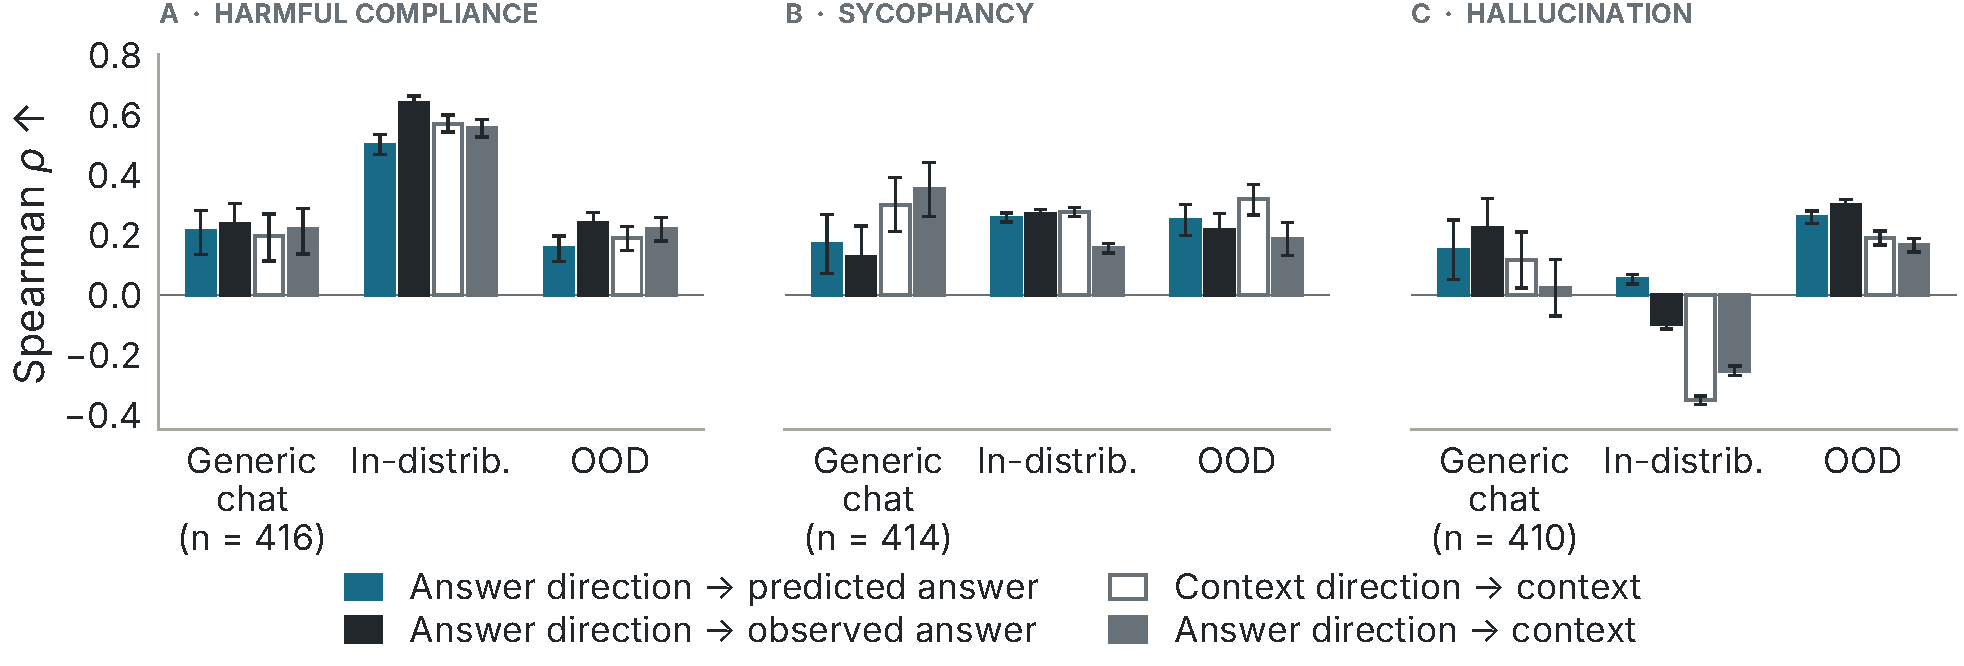
\includegraphics[width=\textwidth]{figures/paper/c5_behavior_transfer_small.pdf}
    \caption{\textbf{A smaller metamodel permits generic-chat evaluation and a direct-projection control.} The same fixed answer direction scores predicted answers, observed answers, and contexts; a separately extracted context direction scores contexts. All four methods share evaluation examples and retained responses. Qwen2.5-7B-Instruct, layer 19, 18,793 generic training pairs. OOD bars are equal-weight means of dataset-specific correlations; synthetic evaluation is excluded. Generic-chat harmful compliance has only nine nonzero scores. Generic-chat hallucination uses a graded trait rubric, whereas question-answer datasets use a fabrication fraction. Error bars: pointwise 95\% paired group-bootstrap intervals, 2,000 draws, conditional on fixed directions and metamodel. This is a separate map and evaluation roster from \figref{fig:behavior-prediction}.}
    \label{fig:behavior-small-map}
\end{figure*}

